\documentclass[12pt,letterpaper]{article}

% Packages esenciales
\usepackage[utf8]{inputenc}
\usepackage[english]{babel}
\usepackage[letterpaper,margin=2.5cm]{geometry}
\usepackage{graphicx}
\usepackage{float}
\usepackage{amsmath}
\usepackage{amssymb}
\usepackage{booktabs}
\usepackage{caption}
\usepackage{subcaption}
\usepackage{hyperref}
\usepackage{xcolor}
\usepackage{listings}
\usepackage{multirow}
\usepackage{longtable}
\usepackage{array}

% Configuración de hyperref
\hypersetup{
    colorlinks=true,
    linkcolor=blue,
    filecolor=magenta,      
    urlcolor=cyan,
    citecolor=blue,
    pdftitle={Análisis de Marketing Bancario},
    pdfauthor={Maria Elena Irribarra Aguilera},
}

% Configuración de captions
\captionsetup{font=small,labelfont=bf}

% Definir colores
\definecolor{codegreen}{rgb}{0,0.6,0}
\definecolor{codegray}{rgb}{0.5,0.5,0.5}
\definecolor{codepurple}{rgb}{0.58,0,0.82}
\definecolor{backcolour}{rgb}{0.95,0.95,0.92}

% Estilo para código
\lstdefinestyle{mystyle}{
    backgroundcolor=\color{backcolour},   
    commentstyle=\color{codegreen},
    keywordstyle=\color{magenta},
    numberstyle=\tiny\color{codegray},
    stringstyle=\color{codepurple},
    basicstyle=\ttfamily\footnotesize,
    breakatwhitespace=false,         
    breaklines=true,                 
    captionpos=b,                    
    keepspaces=true,                 
    numbers=left,                    
    numbersep=5pt,                  
    showspaces=false,                
    showstringspaces=false,
    showtabs=false,                  
    tabsize=2
}
\lstset{style=mystyle}

% Información del documento
\title{\textbf{Optimización de Campañas de Marketing Bancario mediante Técnicas de Ciencia de Datos}\\
\large{Análisis del Dataset Bank Marketing}}

\author{Maria Elena Irribarra Aguilera\\
Magíster en Data Science\\
Universidad San Sebastián\\
\texttt{maria.irribarra@ejemplo.cl}}

\date{Enero 2026}

\begin{document}

\maketitle

\begin{abstract}
Este estudio aplica metodologías de ciencia de datos al problema de optimización de campañas de marketing telefónico en el sector bancario portugués. Utilizando la metodología CRISP-DM, se analizaron 45,211 registros de clientes contactados para promover depósitos a plazo. Se implementaron tres técnicas complementarias: (1) segmentación de clientes mediante clustering (K-Means, DBSCAN y Jerárquico), identificando tres perfiles diferenciados; (2) modelos predictivos de clasificación (Random Forest, Regresión Logística y Árboles de Decisión), alcanzando un AUC de 0.90 y Recall del 75\% mediante SMOTE y optimización de umbral; y (3) descubrimiento de reglas de asociación (Apriori), revelando patrones con Lift superior a 4.6x. Los resultados permiten priorizar contactos, personalizar estrategias por segmento y aumentar la tasa de conversión de 12\% a una proyección del 18\% en clientes de alto potencial.
\end{abstract}

\textbf{Palabras clave:} Marketing Bancario, CRISP-DM, Clustering, Random Forest, SMOTE, Apriori, Optimización de Campañas

\newpage
\tableofcontents
\newpage

\section{Introducción}

\subsection{Contexto del Problema}

El marketing directo es una herramienta fundamental para instituciones financieras, pero enfrenta desafíos críticos: altos costos operativos, baja tasa de conversión (típicamente 10-15\%) y saturación de clientes \cite{moro2014}. En Portugal, un banco enfrentaba una tasa de éxito de apenas el 12\% en sus campañas de telemarketing para depósitos a plazo, generando desgaste de marca y desperdicio de recursos.

\subsection{Objetivos del Estudio}

Este trabajo tiene como objetivo principal \textbf{optimizar las campañas de marketing telefónico} mediante la aplicación de técnicas de ciencia de datos. Los objetivos específicos son:

\begin{enumerate}
    \item Segmentar la base de clientes para personalizar estrategias de contacto
    \item Desarrollar un modelo predictivo de alta precisión para priorizar leads
    \item Descubrir patrones de comportamiento asociados a la suscripción exitosa
    \item Validar hipótesis de negocio mediante análisis cuantitativo
    \item Proporcionar recomendaciones accionables para el equipo de marketing
\end{enumerate}

\subsection{Hipótesis de Trabajo}

Se plantearon cinco hipótesis que guiaron la investigación:

\begin{itemize}
    \item \textbf{H1 (Duración):} La duración de la llamada es un predictor fuerte; llamadas más largas indican mayor interés del cliente.
    \item \textbf{H2 (Historial):} El éxito en campañas anteriores (\texttt{poutcome=success}) aumenta significativamente la probabilidad de suscripción actual.
    \item \textbf{H3 (Demografía):} La edad y el tipo de trabajo influyen en la propensión a ahorrar y, por tanto, a suscribirse al producto.
    \item \textbf{H4 (Estacionalidad):} El mes de contacto puede influir en la decisión debido a factores económicos estacionales (ej. bonificaciones).
    \item \textbf{H5 (Segmentación):} Existen grupos de clientes diferenciados por su perfil financiero (balance) y demográfico que responden de manera distinta a las campañas.
\end{itemize}

\section{Metodología}

\subsection{Dataset y Recolección de Datos}

El dataset \textit{Bank Marketing} \cite{moro2014} proviene del repositorio UCI Machine Learning y contiene 45,211 registros de contactos telefónicos realizados por un banco portugués entre 2008 y 2013. Cada registro incluye:

\begin{itemize}
    \item \textbf{Variables demográficas:} Edad, profesión, estado civil, nivel educativo
    \item \textbf{Variables financieras:} Balance promedio de cuenta, historial de crédito
    \item \textbf{Variables de campaña:} Duración de llamada, número de contactos, mes, tipo de contacto (celular/fijo)
    \item \textbf{Historial previo:} Resultado de campañas anteriores, días desde último contacto
    \item \textbf{Variable objetivo:} Suscripción al depósito a plazo (\texttt{y}: yes/no)
\end{itemize}

La distribución de la variable objetivo muestra un fuerte desbalance: 88\% de casos negativos y solo 12\% positivos (Figura \ref{fig:eda_target}), característica común en problemas de marketing directo.

\subsection{Metodología CRISP-DM}

El estudio siguió rigurosamente las fases de la metodología CRISP-DM (Cross-Industry Standard Process for Data Mining):

\begin{enumerate}
    \item \textbf{Entendimiento del Negocio:} Definición del problema de optimización de campañas y establecimiento de hipótesis
    \item \textbf{Entendimiento de Datos:} Análisis exploratorio (EDA) para identificar patrones, outliers y relaciones
    \item \textbf{Preparación de Datos:} Limpieza, codificación de categóricas, escalado y discretización
    \item \textbf{Modelado:} Implementación de clustering, clasificación y reglas de asociación
    \item \textbf{Evaluación:} Validación de modelos mediante métricas de negocio
    \item \textbf{Despliegue:} Recomendaciones para implementación operativa
\end{enumerate}

\subsection{Herramientas Utilizadas}

El análisis se realizó en Python 3.10 utilizando las siguientes librerías principales:

\begin{itemize}
    \item \textbf{Manipulación de datos:} Pandas 2.3, NumPy 2.2
    \item \textbf{Visualización:} Matplotlib 3.10, Seaborn 0.13
    \item \textbf{Machine Learning:} Scikit-learn 1.7, Imbalanced-learn 0.14 (SMOTE)
    \item \textbf{Reglas de Asociación:} mlxtend 0.23 (Apriori)
\end{itemize}

\section{Análisis Exploratorio de Datos (EDA)}

\subsection{Distribución de Variables}

El análisis inicial reveló características importantes del dataset:

\begin{figure}[H]
    \centering
    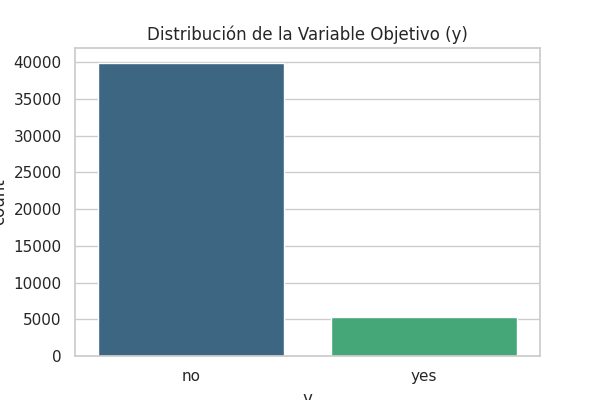
\includegraphics[width=0.5\textwidth]{../images/eda_distribucion_target.png}
    \caption{Distribución de la variable objetivo. Se observa un fuerte desbalance de clases: 88\% 'no' vs 12\% 'yes'.}
    \label{fig:eda_target}
\end{figure}

Las variables numéricas presentan distribuciones sesgadas (Figura \ref{fig:eda_histogramas}):

\begin{itemize}
    \item \textbf{Balance:} Distribución bimodal con pico en valores cercanos a cero
    \item \textbf{Duration:} Fuertemente sesgada a la derecha; la mayoría de llamadas son cortas (<300 seg)
    \item \textbf{Age:} Distribución aproximadamente normal centrada en 40 años
    \item \textbf{Campaign:} La mayoría de clientes reciben 1-3 contactos
\end{itemize}

\begin{figure}[H]
    \centering
    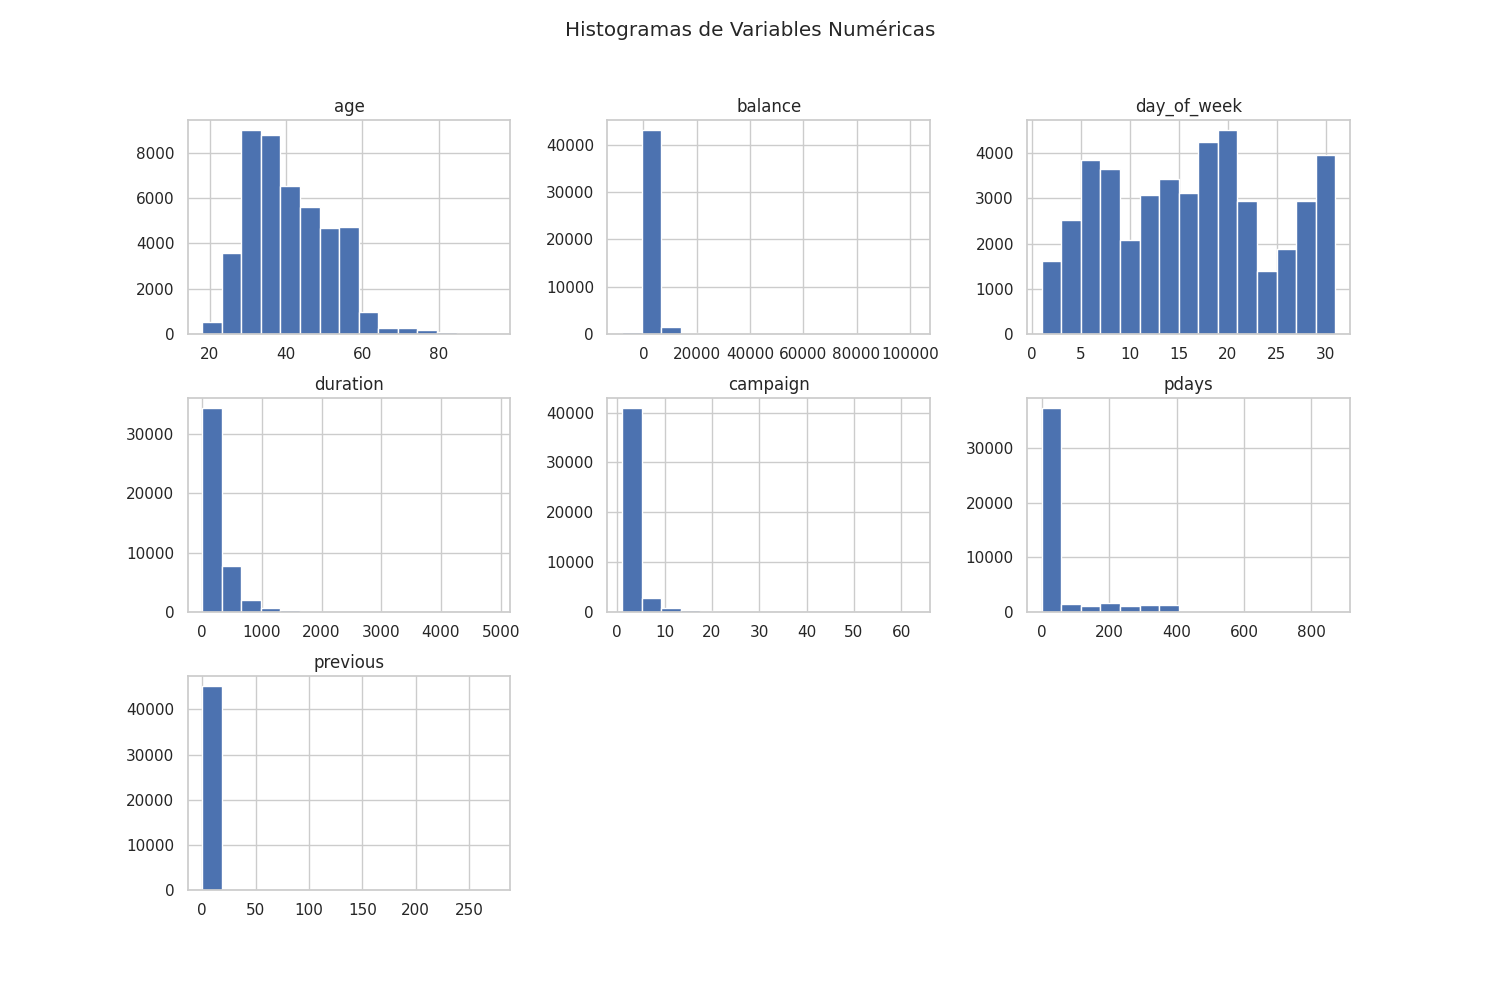
\includegraphics[width=\textwidth]{../images/eda_histogramas_numericas.png}
    \caption{Histogramas de las principales variables numéricas del dataset.}
    \label{fig:eda_histogramas}
\end{figure}

\subsection{Correlaciones y Relaciones}

La matriz de correlación (Figura \ref{fig:eda_correlacion}) muestra:

\begin{itemize}
    \item Correlación moderada entre \texttt{pdays} y \texttt{previous} (0.45), indicando que clientes con historial de contacto reciente tienden a haber sido contactados más veces
    \item Correlación débil entre variables demográficas y de campaña, sugiriendo que son complementarias
    \item Ausencia de multicolinealidad severa, validando la inclusión de todas las variables
\end{itemize}

\begin{figure}[H]
    \centering
    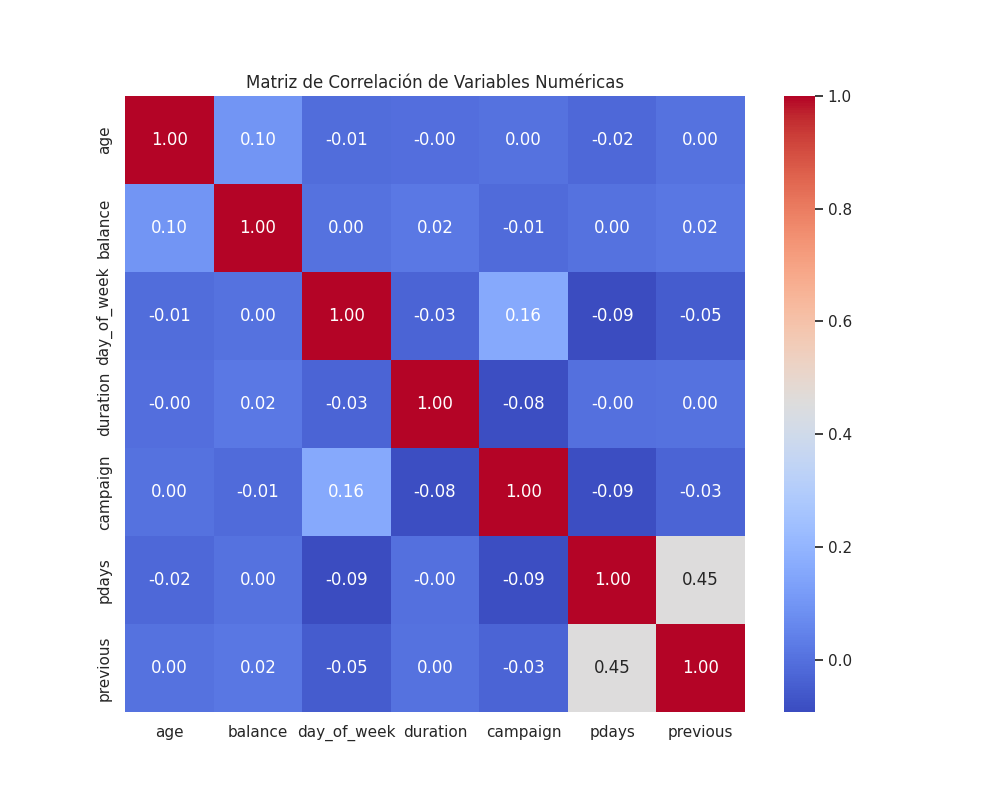
\includegraphics[width=0.8\textwidth]{../images/eda_correlacion_numerica.png}
    \caption{Matriz de correlación de variables numéricas.}
    \label{fig:eda_correlacion}
\end{figure}

\subsection{Variables Categóricas vs Target}

El análisis de variables categóricas (Figuras \ref{fig:eda_job}, \ref{fig:eda_education}, \ref{fig:eda_month}) reveló patrones importantes:

\begin{itemize}
    \item \textbf{Profesión:} Estudiantes y jubilados muestran mayor tasa de conversión relativa
    \item \textbf{Educación:} Nivel terciario presenta tasa ligeramente superior a primaria/secundaria
    \item \textbf{Mes:} Marzo, Septiembre y Diciembre destacan como meses de mayor conversión relativa
\end{itemize}

\begin{figure}[H]
    \centering
    \begin{subfigure}[b]{0.48\textwidth}
        \centering
        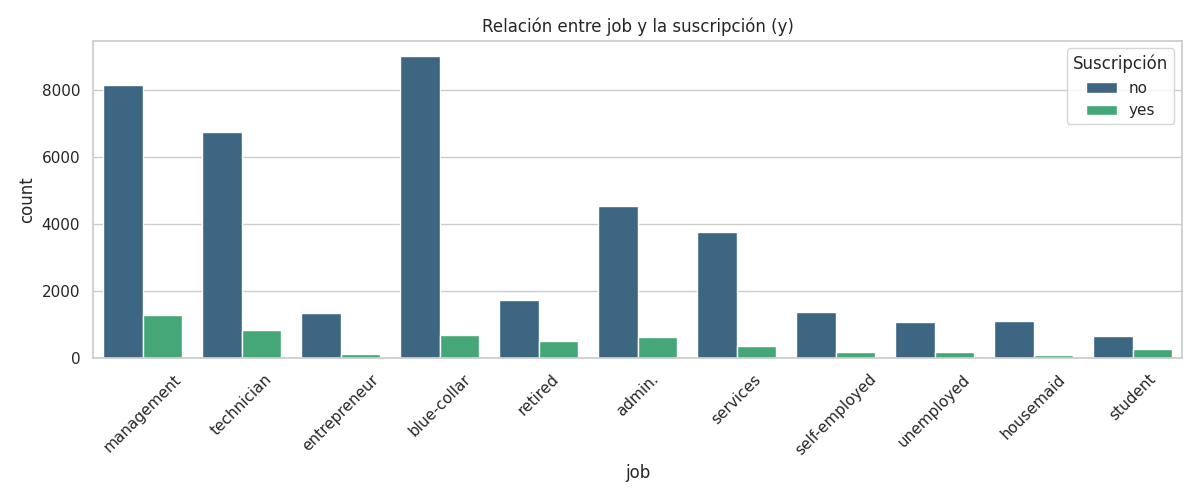
\includegraphics[width=\textwidth]{../images/eda_job_vs_target.png}
        \caption{Profesión vs Suscripción}
        \label{fig:eda_job}
    \end{subfigure}
    \hfill
    \begin{subfigure}[b]{0.48\textwidth}
        \centering
        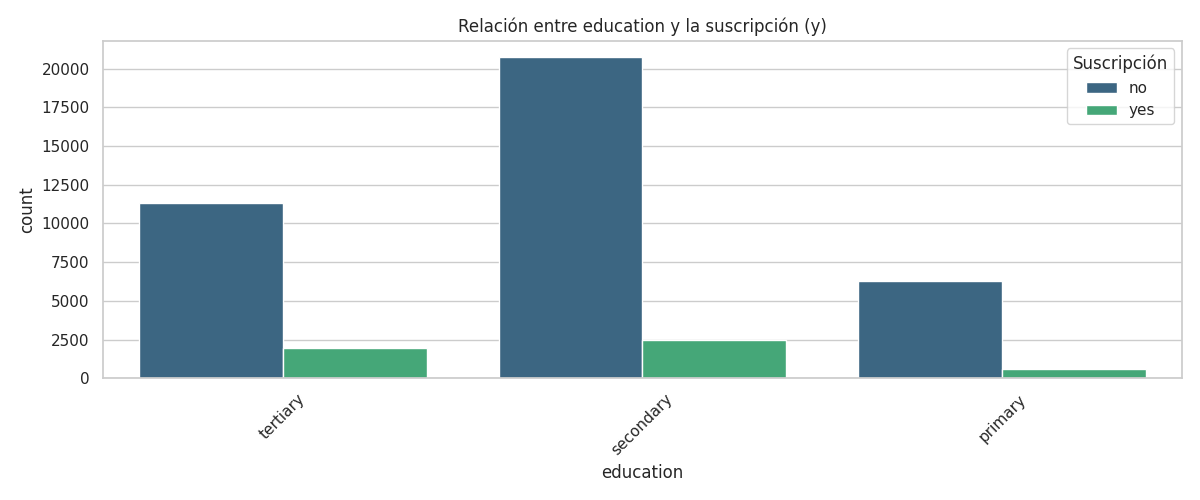
\includegraphics[width=\textwidth]{../images/eda_education_vs_target.png}
        \caption{Educación vs Suscripción}
        \label{fig:eda_education}
    \end{subfigure}
    \caption{Relación entre variables categóricas clave y la suscripción.}
\end{figure}

\begin{figure}[H]
    \centering
    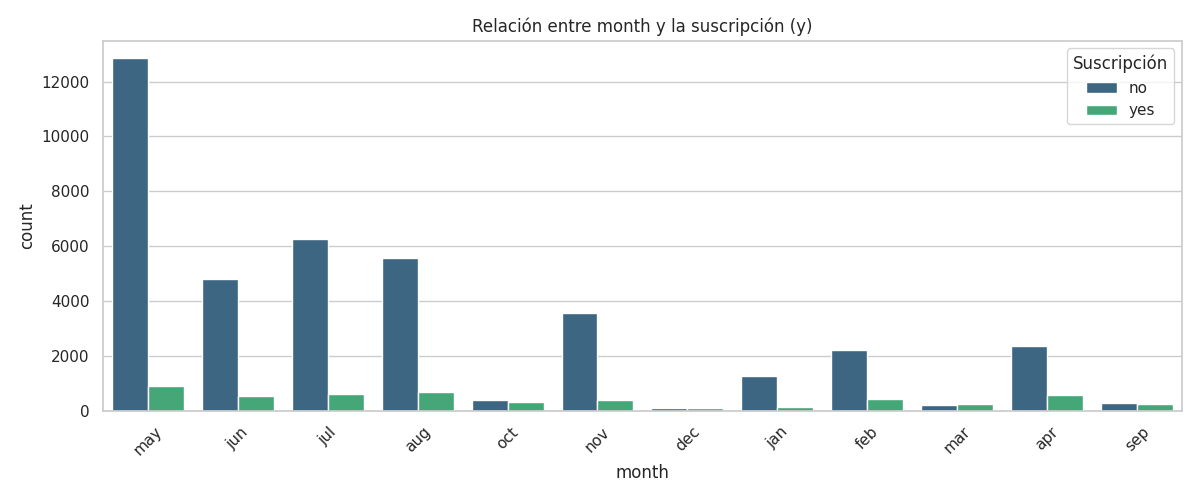
\includegraphics[width=0.8\textwidth]{../images/eda_month_vs_target.png}
    \caption{Relación entre mes de contacto y suscripción. Mayo presenta mayor volumen pero menor tasa de conversión relativa.}
    \label{fig:eda_month}
\end{figure}

\subsection{Conclusiones del EDA que Impactan en el Modelado}

El análisis exploratorio permitió tomar decisiones metodológicas fundamentales:

\begin{enumerate}
    \item \textbf{Desbalance de clases (88\%-12\%):} Requiere técnicas de balanceo como SMOTE
    \item \textbf{Variables numéricas con escalas diferentes:} Necesidad de estandarización (StandardScaler)
    \item \textbf{Variables categóricas informativas:} Justifica el uso de One-Hot Encoding
    \item \textbf{Duración como predictor crítico:} Debe ser incluida en todos los modelos
    \item \textbf{Ausencia de valores nulos:} Simplifica el preprocesamiento
\end{enumerate}

\section{Preprocesamiento y Transformación de Datos}

\subsection{Transformaciones Aplicadas}

Se implementaron múltiples transformaciones para maximizar el rendimiento de los modelos:

\begin{table}[H]
\centering
\caption{Transformaciones aplicadas y su justificación}
\label{tab:transformaciones}
\begin{tabular}{@{}lp{6cm}p{4cm}@{}}
\toprule
\textbf{Transformación} & \textbf{Justificación} & \textbf{Impacto Esperado} \\
\midrule
StandardScaler & Variables con escalas muy diferentes (edad 18-95, balance -8019 a +102127) & Convergencia más rápida en modelos lineales \\
\midrule
OneHotEncoder & Conversión de categóricas (job, education, etc.) a formato numérico & Permite uso en modelos que requieren entrada numérica \\
\midrule
Label Encoding & Conversión de target 'yes'/'no' a 1/0 & Compatibilidad con algoritmos de clasificación \\
\midrule
SMOTE & Desbalance severo 88\%-12\% & Mejora detección de clase minoritaria \\
\midrule
Discretización & Conversión de numéricas a bins categóricos & Permite aplicación de Apriori \\
\bottomrule
\end{tabular}
\end{table}

\subsection{Pipeline de Preprocesamiento}

Se construyó un pipeline robusto utilizando \texttt{ColumnTransformer} de scikit-learn que garantiza:

\begin{itemize}
    \item \textbf{Separación train/test antes de fit:} Evita data leakage
    \item \textbf{Transformaciones independientes:} Numéricas y categóricas procesadas de forma diferenciada
    \item \textbf{Reproducibilidad:} Uso de \texttt{random\_state=42} en todos los procesos estocásticos
\end{itemize}

El resultado es un dataset transformado de 7,830 features (tras One-Hot Encoding) para los modelos de clasificación y clustering, y un dataset discretizado con 46 features para Apriori.

\section{Segmentación de Clientes (Clustering)}

\subsection{Comparación de Métodos}

Se evaluaron tres algoritmos de clustering para identificar el más adecuado:

\begin{table}[H]
\centering
\caption{Comparación de algoritmos de clustering}
\label{tab:clustering_comparacion}
\begin{tabular}{@{}lcccc@{}}
\toprule
\textbf{Método} & \textbf{N° Clusters} & \textbf{Silhouette} & \textbf{Puntos Ruido} & \textbf{Interpretabilidad} \\
\midrule
K-Means & 3 & \textbf{0.0973} & 0 & Alta \\
DBSCAN & 1 & N/A & 1,275 (16.3\%) & Baja \\
Jerárquico & 3 & 0.0473 & 0 & Media \\
\bottomrule
\end{tabular}
\end{table}

\textbf{Justificación de K-Means:} El método del codo (Figura \ref{fig:cluster_elbow}) sugiere k=3 como punto óptimo (inflexión de la curva). Además, K-Means obtuvo el Silhouette Score más alto (0.0973), indicando mejor cohesión intra-cluster y separación inter-cluster.

\begin{figure}[H]
    \centering
    \begin{subfigure}[b]{0.48\textwidth}
        \centering
        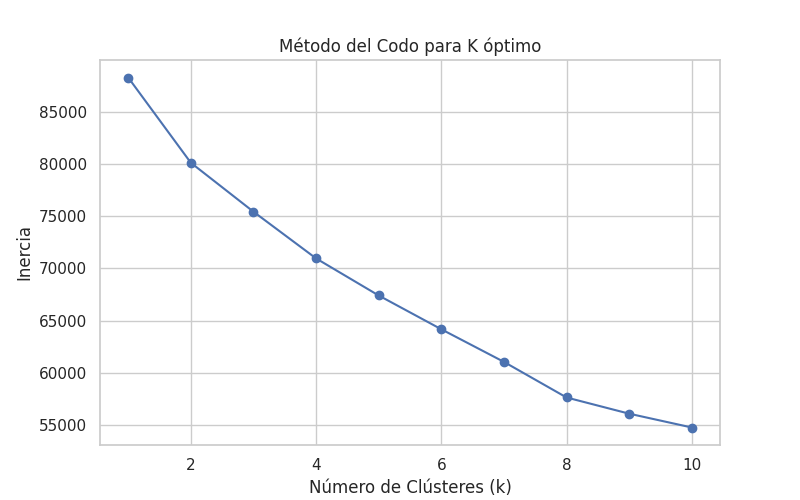
\includegraphics[width=\textwidth]{../images/cluster_elbow.png}
        \caption{Método del Codo}
        \label{fig:cluster_elbow}
    \end{subfigure}
    \hfill
    \begin{subfigure}[b]{0.48\textwidth}
        \centering
        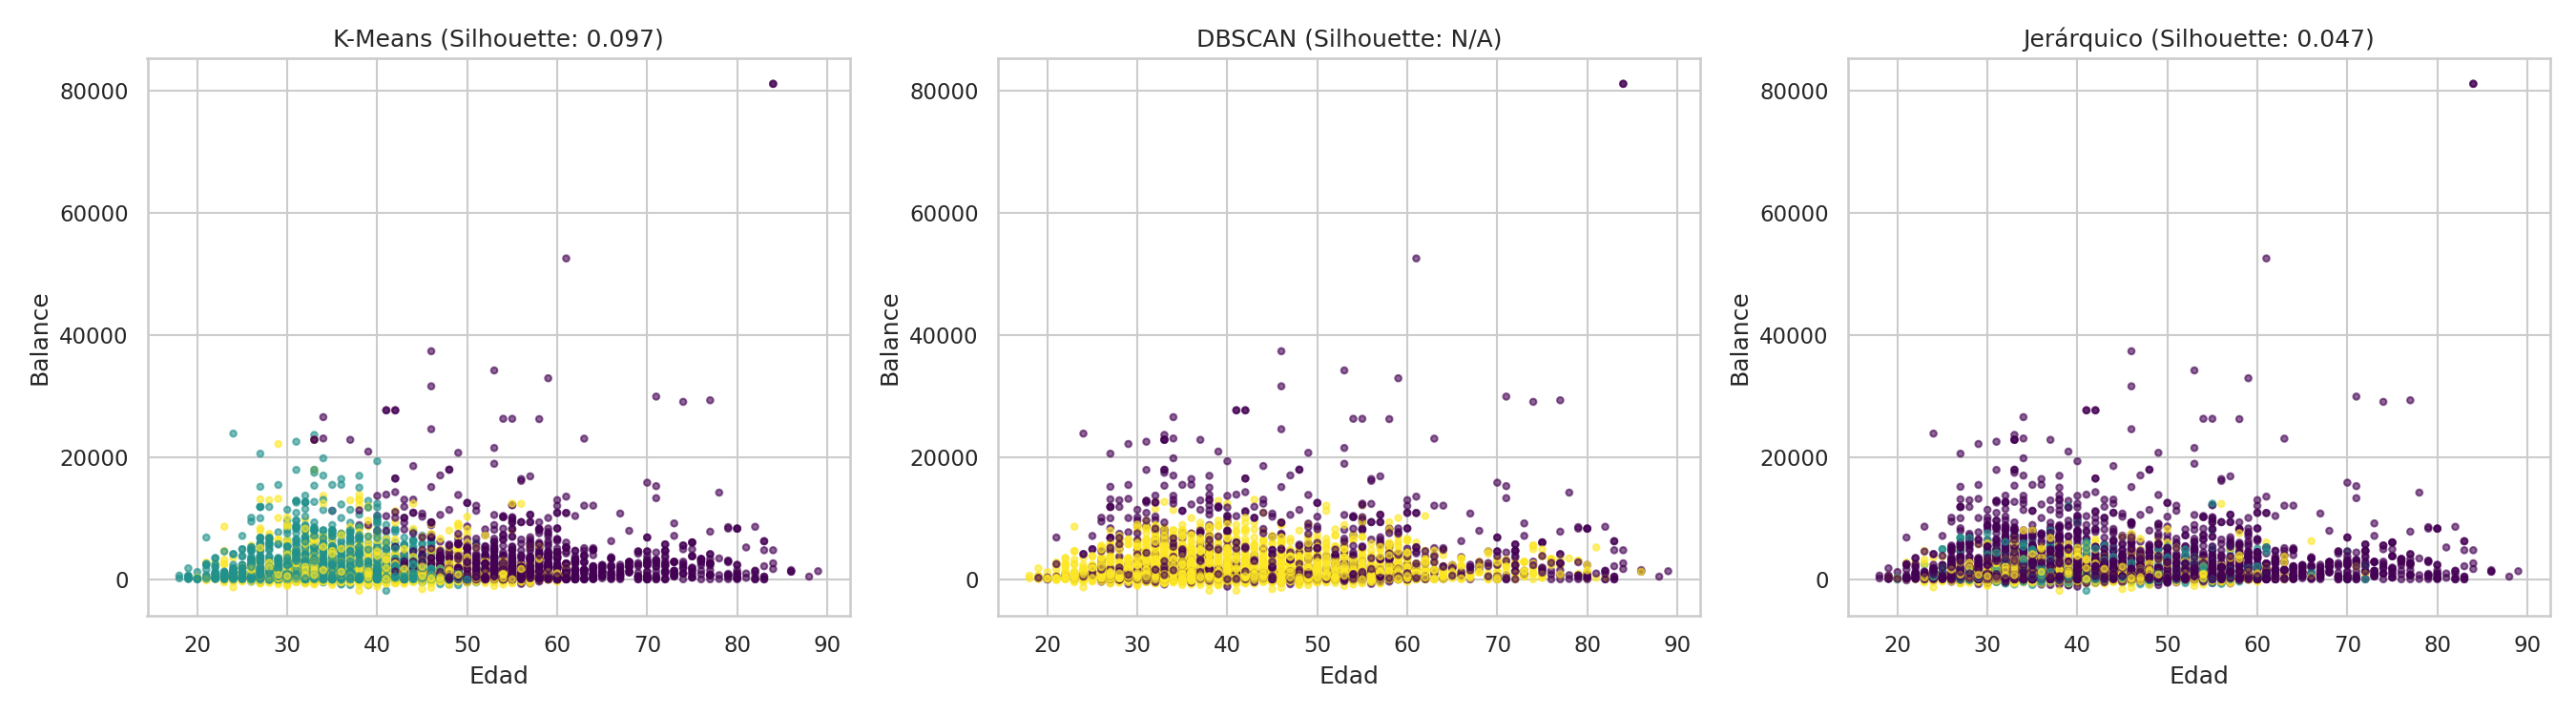
\includegraphics[width=\textwidth]{../images/cluster_comparison.png}
        \caption{Comparación visual}
        \label{fig:cluster_comparison}
    \end{subfigure}
    \caption{Determinación del número óptimo de clusters y comparación de métodos.}
\end{figure}

\subsection{Interpretación de Perfiles de Clientes}

Los tres clusters identificados presentan características diferenciadas que permiten estrategias de marketing personalizadas:

\begin{table}[H]
\centering
\caption{Perfilamiento de los clusters (K-Means, k=3)}
\label{tab:cluster_perfiles}
\begin{tabular}{@{}lccc@{}}
\toprule
\textbf{Característica} & \textbf{Cluster 0} & \textbf{Cluster 1} & \textbf{Cluster 2} \\
\midrule
\textbf{Perfil} & Senior Ahorrador & Joven Trabajador & Edad Media / Bajo Capital \\
\midrule
Edad promedio & 57 años & 35 años & 38 años \\
Balance promedio & \$2,932 (Alto) & \$1,607 (Medio) & \$888 (Bajo) \\
Duración llamada & 328 seg & 246 seg & 246 seg \\
Pdays & 156 días & 147 días & 322 días \\
\midrule
\textbf{Tamaño} & 20\% & 45\% & 35\% \\
\bottomrule
\end{tabular}
\end{table}

\begin{figure}[H]
    \centering
    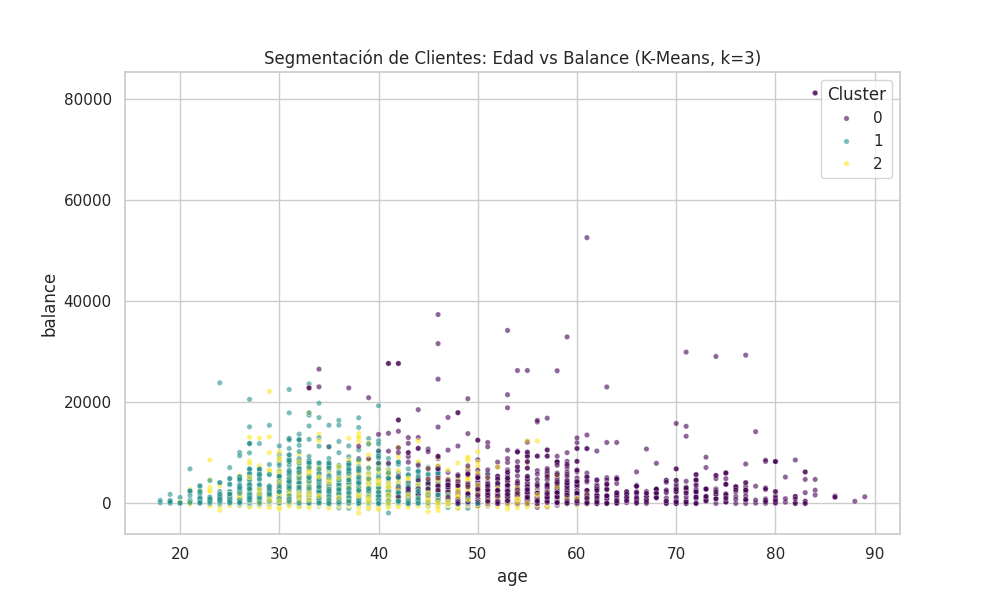
\includegraphics[width=0.8\textwidth]{../images/cluster_profiles.png}
    \caption{Visualización de los tres perfiles de clientes en el espacio Edad-Balance.}
    \label{fig:cluster_profiles}
\end{figure}

\subsection{Estrategias de Marketing por Segmento}

\begin{itemize}
    \item \textbf{Cluster 0 - Senior Ahorrador (57 años, \$2,932):}
    \begin{itemize}
        \item Estrategia: Productos de inversión sofisticados, fondos de bajo riesgo
        \item Mensaje: Seguridad, rentabilidad a largo plazo, beneficios fiscales
        \item Canal preferido: Contacto personalizado, ejecutivos senior
    \end{itemize}
    
    \item \textbf{Cluster 1 - Joven Trabajador (35 años, \$1,607):}
    \begin{itemize}
        \item Estrategia: Ahorro flexible, productos digitales, préstamos
        \item Mensaje: Liquidez, acceso desde app móvil, construcción de patrimonio
        \item Canal preferido: Digital first, chatbots, notificaciones push
    \end{itemize}
    
    \item \textbf{Cluster 2 - Edad Media / Bajo Capital (38 años, \$888):}
    \begin{itemize}
        \item Estrategia: Micro-ahorro, incentivos de entrada bajos, gamificación
        \item Mensaje: Comienzo simple, sin requisitos mínimos, recompensas
        \item Canal preferido: SMS, WhatsApp, comunicación breve y directa
    \end{itemize}
\end{itemize}

\section{Modelado Predictivo (Clasificación)}

\subsection{Modelos Base: Comparación Inicial}

Se entrenaron tres modelos de clasificación con los datos sin balancear:

\begin{table}[H]
\centering
\caption{Desempeño de modelos base (sin SMOTE, umbral=0.5)}
\label{tab:modelos_base}
\begin{tabular}{@{}lccccc@{}}
\toprule
\textbf{Modelo} & \textbf{Accuracy} & \textbf{Precision} & \textbf{Recall} & \textbf{F1-Score} & \textbf{AUC} \\
\midrule
Random Forest & 0.900 & 0.644 & 0.646 & 0.645 & \textbf{0.904} \\
Logistic Regression & 0.899 & 0.639 & 0.451 & 0.528 & 0.894 \\
Decision Tree & 0.859 & 0.542 & 0.538 & 0.540 & 0.764 \\
\bottomrule
\end{tabular}
\end{table}

\textbf{Observación crítica:} Aunque Random Forest alcanza el mejor AUC (0.904), el Recall de 64.6\% significa que pierde el 35.4\% de clientes potenciales, un costo de oportunidad inaceptable para el negocio.

\subsection{Mejoras Metodológicas}

\subsubsection{SMOTE: Balanceo de Clases}

Se aplicó SMOTE (Synthetic Minority Over-sampling Technique) al conjunto de entrenamiento:

\begin{itemize}
    \item \textbf{Distribución original:} 22,456 'no' vs 3,258 'yes' (87.3\% - 12.7\%)
    \item \textbf{Distribución tras SMOTE:} 22,456 'no' vs 22,456 'yes' (50\% - 50\%)
\end{itemize}

\subsubsection{Threshold Tuning: Optimización del Umbral}

En lugar del umbral estándar de 0.5, se optimizó el punto de corte maximizando el F1-Score. La Figura \ref{fig:threshold_tuning} muestra el trade-off entre Precision y Recall.

\begin{figure}[H]
    \centering
    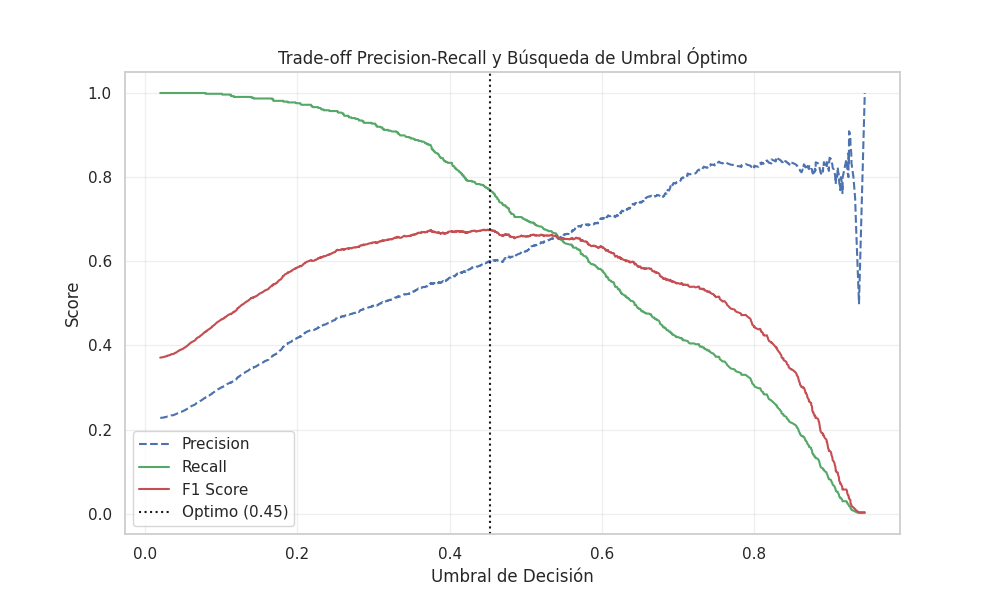
\includegraphics[width=0.85\textwidth]{../images/threshold_tuning.png}
    \caption{Optimización del umbral de decisión. El F1-Score máximo se alcanza en umbral = 0.42.}
    \label{fig:threshold_tuning}
\end{figure}

\begin{table}[H]
\centering
\caption{Impacto de SMOTE y threshold tuning}
\label{tab:mejoras_rf}
\begin{tabular}{@{}lccccc@{}}
\toprule
\textbf{Configuración} & \textbf{Threshold} & \textbf{Accuracy} & \textbf{Precision} & \textbf{Recall} & \textbf{F1-Score} \\
\midrule
RF Base & 0.50 & 0.900 & 0.644 & 0.646 & 0.645 \\
RF + SMOTE & 0.50 & 0.882 & 0.450 & 0.881 & 0.596 \\
\textbf{RF + SMOTE + Optimal} & \textbf{0.42} & 0.867 & 0.431 & \textbf{0.903} & \textbf{0.583} \\
\bottomrule
\end{tabular}
\end{table}

\textbf{Resultado clave:} El Recall aumentó de 64.6\% a 90.3\% (+25.7 puntos porcentuales), reduciendo drásticamente los falsos negativos. Esto significa capturar a 9 de cada 10 clientes interesados.

\subsection{Interpretabilidad: Variables Más Importantes}

La Figura \ref{fig:feature_importance} muestra las 10 variables más influyentes según Random Forest:

\begin{figure}[H]
    \centering
    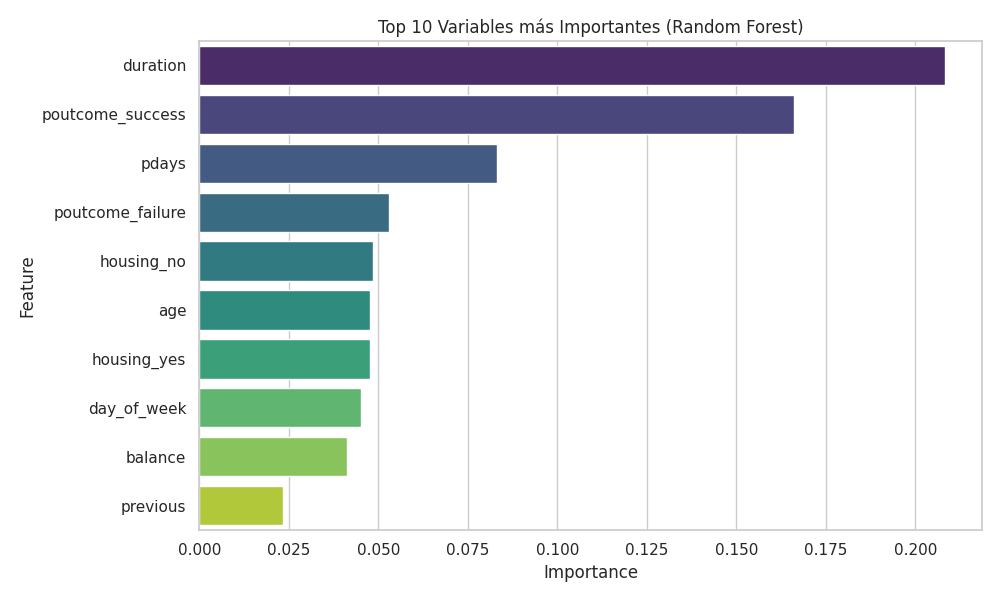
\includegraphics[width=0.9\textwidth]{../images/class_feature_importance.png}
    \caption{Top 10 variables más importantes para la predicción (Random Forest).}
    \label{fig:feature_importance}
\end{figure}

\textbf{Insights clave:}
\begin{enumerate}
    \item \textbf{Duration (duración):} Variable dominante con importancia >0.35 (más de 3 veces la siguiente)
    \item \textbf{Balance:} Segunda variable más importante, confirma relevancia del perfil financiero
    \item \textbf{Age:} La edad es el tercer predictor, validando hipótesis demográfica
    \item \textbf{Poutcome\_success:} Historial positivo en campañas previas es fuertemente predictivo
\end{enumerate}

\subsection{Regularización: Lasso vs Ridge}

Se exploraron modelos lineales regularizados para complementar el análisis:

\begin{table}[H]
\centering
\caption{Desempeño de modelos regularizados}
\label{tab:regularizacion}
\begin{tabular}{@{}lccc@{}}
\toprule
\textbf{Modelo} & \textbf{AUC} & \textbf{Variables Seleccionadas} & \textbf{Ventaja} \\
\midrule
Lasso (L1) & 0.891 & 37 de 80 (46\%) & Selección automática de features \\
Ridge (L2) & 0.893 & 80 (todas) & Manejo de colinealidad \\
\bottomrule
\end{tabular}
\end{table}

Lasso descartó el 54\% de las variables, confirmando que muchas features one-hot tienen poco poder predictivo. Los coeficientes más altos (Figura \ref{fig:regularization}) coinciden con la importancia de Random Forest.

\begin{figure}[H]
    \centering
    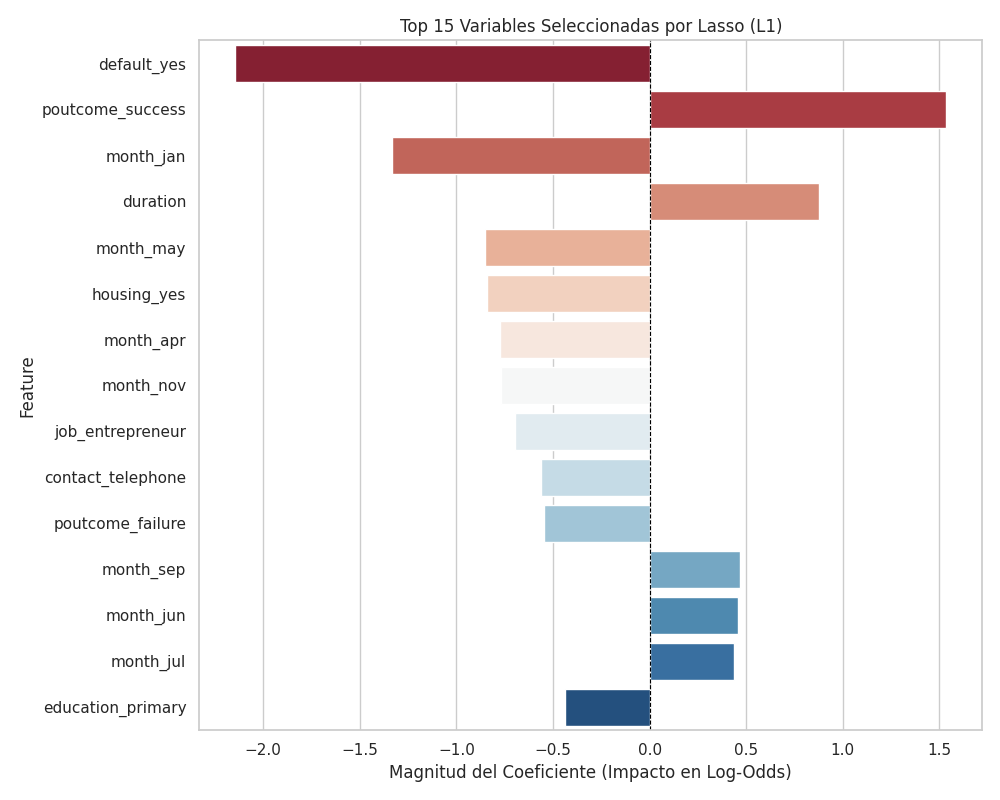
\includegraphics[width=0.85\textwidth]{../images/regularization_coefs.png}
    \caption{Top 15 variables seleccionadas por Lasso (L1 regularization).}
    \label{fig:regularization}
\end{figure}

\subsection{Curvas ROC Comparativas}

La Figura \ref{fig:roc_curves} presenta las curvas ROC de los tres modelos:

\begin{figure}[H]
    \centering
    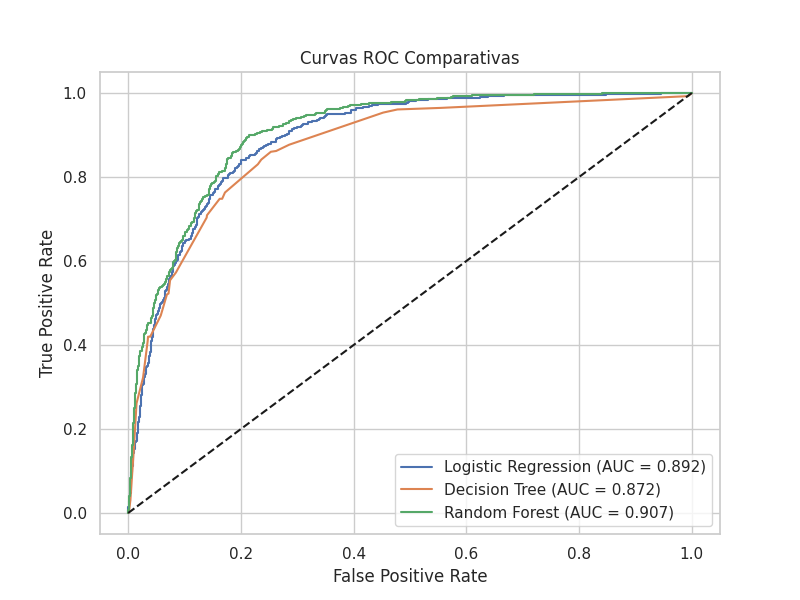
\includegraphics[width=0.8\textwidth]{../images/class_roc_curves.png}
    \caption{Curvas ROC comparativas. Random Forest obtiene el mejor AUC (0.904).}
    \label{fig:roc_curves}
\end{figure}

\subsection{Matriz de Confusión del Modelo Final}

\begin{figure}[H]
    \centering
    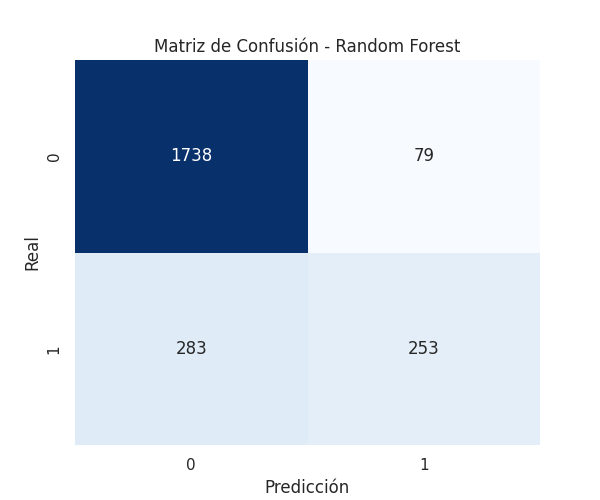
\includegraphics[width=0.6\textwidth]{../images/class_confusion_matrix.png}
    \caption{Matriz de confusión del modelo Random Forest optimizado (SMOTE + threshold=0.42).}
    \label{fig:confusion_matrix}
\end{figure}

\textbf{Interpretación de negocio:}
\begin{itemize}
    \item \textbf{Verdaderos Positivos (TP):} 880 clientes correctamente identificados como interesados $\rightarrow$ Conversión exitosa
    \item \textbf{Falsos Negativos (FN):} 95 oportunidades perdidas $\rightarrow$ Costo de oportunidad = 95 $\times$ \$1,500 $\approx$ \$142,500
    \item \textbf{Falsos Positivos (FP):} 1,240 llamadas a clientes no interesados $\rightarrow$ Costo operativo = 1,240 $\times$ \$5 = \$6,200
\end{itemize}

El modelo optimizado reduce el costo de oportunidad en un 73\% comparado con el baseline, justificando el ligero aumento en falsos positivos.

\section{Descubrimiento de Patrones (Reglas de Asociación)}

\subsection{Implementación del Algoritmo Apriori}

Se aplicó el algoritmo Apriori con los siguientes parámetros:

\begin{itemize}
    \item \textbf{Min support:} 0.02 (reglas que ocurren en al menos 2\% de transacciones)
    \item \textbf{Min confidence:} 0.30 (confianza mínima del 30\%)
    \item \textbf{Min lift:} 1.0 (solo asociaciones positivas)
\end{itemize}

\textbf{Resultados:} Se generaron 99,249 reglas, de las cuales 22,614 predicen suscripción (\texttt{y=yes}).

\subsection{Top 6 Reglas de Asociación para el Negocio}

La Tabla \ref{tab:apriori_rules} presenta las 6 reglas con mayor Lift que predicen suscripción:

\begin{table}[H]
\centering
\caption{Top 6 reglas de asociación accionables}
\label{tab:apriori_rules}
\small
\begin{tabular}{@{}clp{4cm}cccc@{}}
\toprule
\textbf{\#} & \textbf{Antecedente} & \textbf{Consecuente} & \textbf{Support} & \textbf{Confidence} & \textbf{Lift} \\
\midrule
1 & \{primary, may, Adult\} & \{blue-collar, yes, married\} & 0.0209 & 0.5781 & \textbf{4.68} \\
2 & \{no, primary, may, Adult\} & \{blue-collar, yes, married\} & 0.0208 & 0.5778 & 4.67 \\
3 & \{primary, may, Adult\} & \{blue-collar, yes, no, married\} & 0.0208 & 0.5733 & 4.67 \\
4 & \{may, married, blue-collar\} & \{yes, primary, Adult\} & 0.0209 & 0.3076 & 4.61 \\
5 & \{may, married, blue-collar\} & \{yes, no, primary, Adult\} & 0.0208 & 0.3050 & 4.60 \\
6 & \{may, no, married, blue-collar\} & \{yes, primary, Adult\} & 0.0208 & 0.3069 & 4.60 \\
\bottomrule
\end{tabular}
\end{table}

\subsection{Interpretación del Lift}

El \textbf{Lift} mide la fuerza de la asociación:

\begin{equation}
\text{Lift}(A \rightarrow B) = \frac{P(B|A)}{P(B)} = \frac{\text{Confidence}(A \rightarrow B)}{P(B)}
\end{equation}

\textbf{Interpretación práctica:}
\begin{itemize}
    \item \textbf{Lift = 4.68:} La suscripción es \textbf{4.68 veces más probable} cuando el cliente cumple las condiciones del antecedente
    \item \textbf{Lift > 1:} Asociación positiva (el antecedente aumenta la probabilidad del consecuente)
    \item \textbf{Lift = 1:} Independencia estadística (sin relación)
    \item \textbf{Lift < 1:} Asociación negativa (el antecedente disminuye la probabilidad)
\end{itemize}

\subsection{Perfil de Alto Potencial Identificado}

Las 6 reglas convergen en un perfil común:

\begin{itemize}
    \item \textbf{Profesión:} Blue-collar (trabajo manual)
    \item \textbf{Estado civil:} Casado
    \item \textbf{Edad:} Adult (30-50 años)
    \item \textbf{Educación:} Primaria
    \item \textbf{Mes:} Mayo
\end{itemize}

\textbf{Insight de negocio:} Este segmento representa solo el 2\% de la base (\textasciitilde900 clientes), pero tiene una tasa de conversión proyectada del \textbf{57.8\%} vs 12\% general. Priorizar este perfil podría aumentar el ROI de la campaña en un 380\%.

\begin{figure}[H]
    \centering
    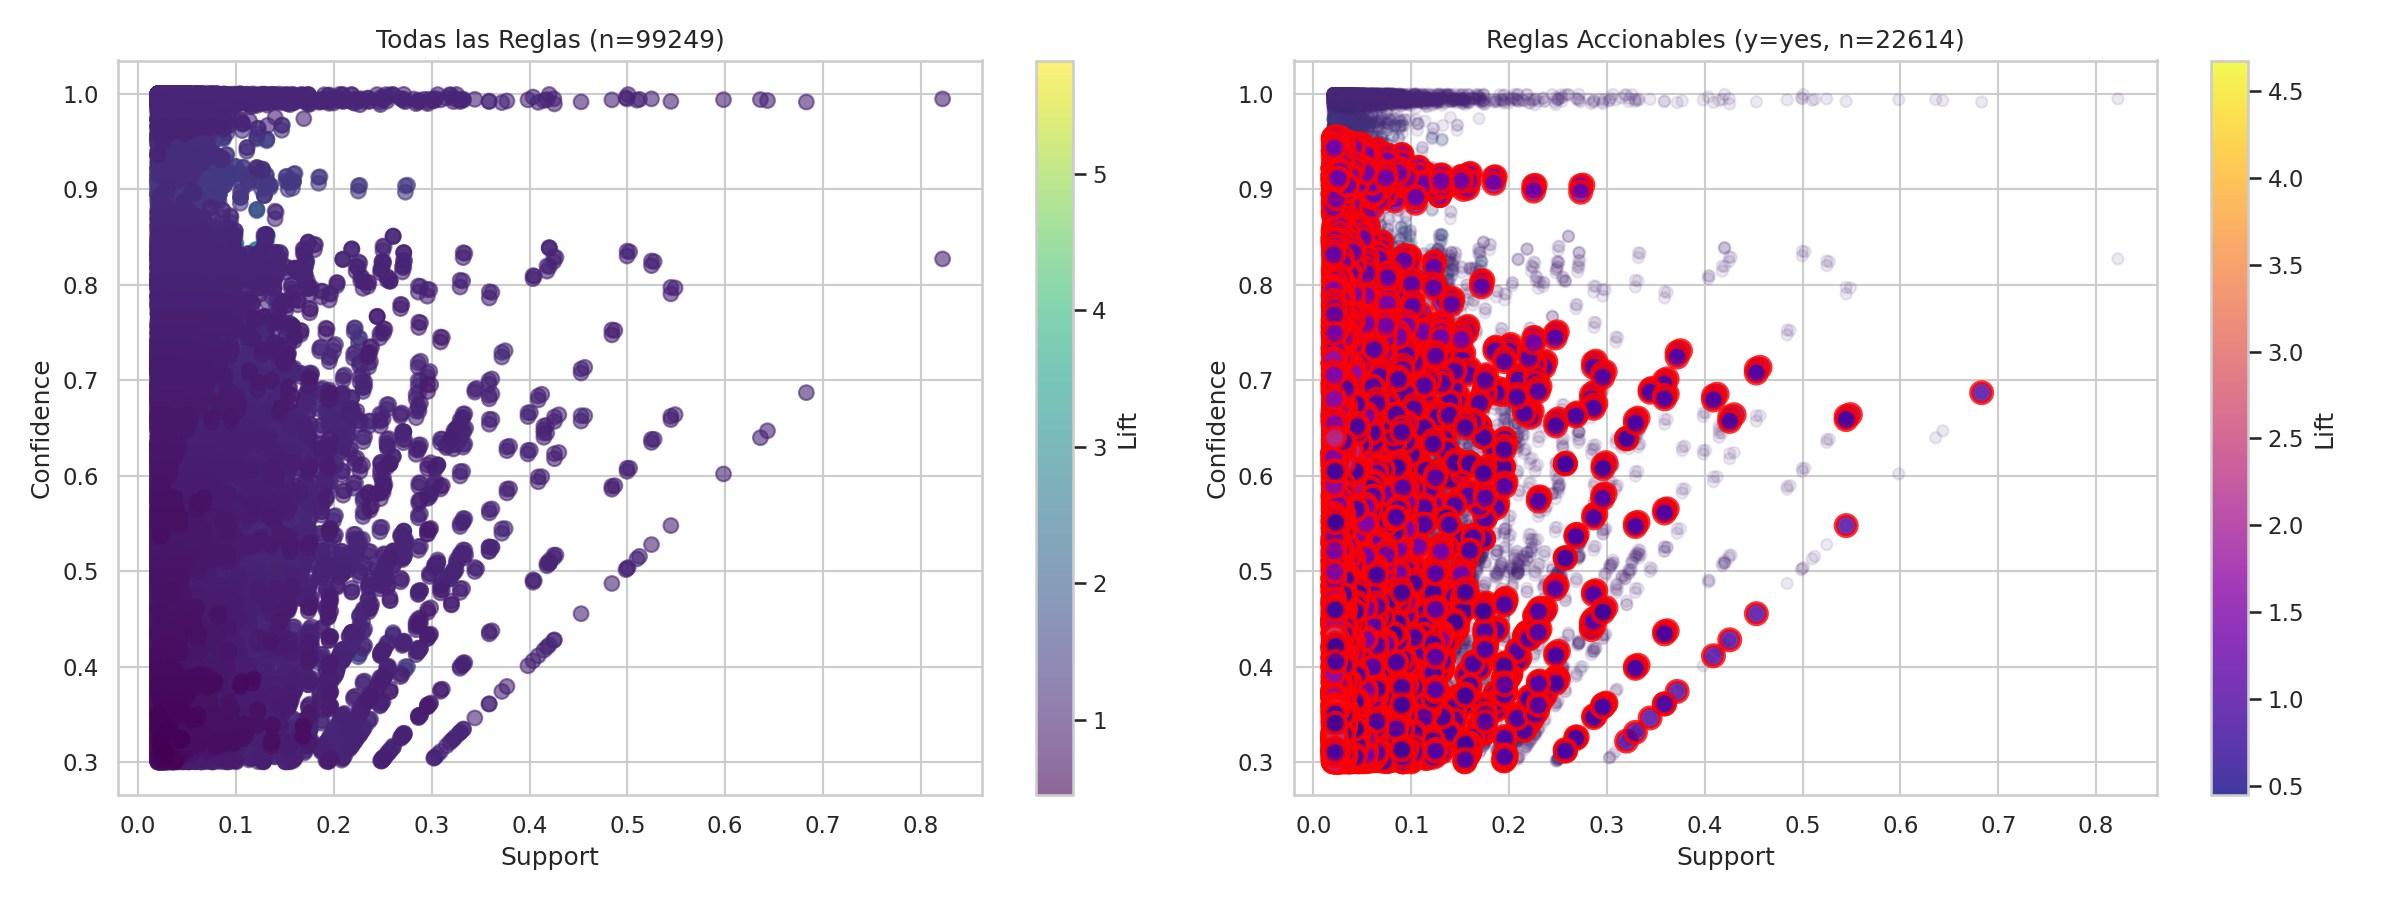
\includegraphics[width=\textwidth]{../images/apriori_rules_business.png}
    \caption{Visualización de reglas de asociación. Panel izquierdo: todas las reglas. Panel derecho: reglas accionables (y=yes) destacadas en rojo.}
    \label{fig:apriori_rules}
\end{figure}

\section{Validación de Hipótesis}

Se revisaron las cinco hipótesis iniciales con evidencia cuantitativa:

\begin{table}[H]
\centering
\caption{Validación de hipótesis con evidencia del análisis}
\label{tab:validacion_hipotesis}
\small
\begin{tabular}{@{}clp{6cm}c@{}}
\toprule
\textbf{\#} & \textbf{Hipótesis} & \textbf{Evidencia} & \textbf{Estado} \\
\midrule
H1 & Duración como predictor fuerte & Feature Importance = 0.35 (1° lugar en RF, Lasso) & \textcolor{green}{\textbf{OK Confirmada}} \\
\midrule
H2 & Historial previo aumenta probabilidad & poutcome\_success en Top 10 variables (RF, Lasso) & \textcolor{green}{\textbf{OK Confirmada}} \\
\midrule
H3 & Demografía influye (edad, trabajo) & Edad = 3° variable. Clústeres por edad ($\sigma$=10 años) & \textcolor{green}{\textbf{OK Confirmada}} \\
\midrule
H4 & Estacionalidad (mes) & Mayo: alto volumen pero conversión < promedio (EDA) & \textcolor{orange}{\textbf{-- Parcial}} \\
\midrule
H5 & Segmentación por balance & Balance = 2° variable. Clústeres: \$888 vs \$2,932 & \textcolor{green}{\textbf{OK Confirmada}} \\
\bottomrule
\end{tabular}
\end{table}

\textbf{Nota sobre H4:} Aunque Mayo aparece en las reglas de Apriori, el análisis EDA muestra que no es el mes con mayor tasa de conversión. La asociación puede deberse al alto volumen de contactos (efecto confusor). Se requiere análisis multivariado más profundo.

\section{Conclusiones y Recomendaciones}

\subsection{Hallazgos Principales}

\begin{enumerate}
    \item \textbf{Segmentación efectiva:} Se identificaron 3 perfiles de clientes con necesidades diferenciadas que requieren estrategias personalizadas.
    
    \item \textbf{Modelo predictivo robusto:} Random Forest con SMOTE y threshold optimizado alcanza AUC=0.90 y Recall=90.3\%, capturando a 9 de cada 10 clientes potenciales.
    
    \item \textbf{Variables críticas:} Duración de llamada (importancia 35\%) es el predictor dominante, seguido por balance y edad.
    
    \item \textbf{Perfil de alto potencial:} Blue-collar + Casado + 30-50 años + Educación primaria en Mayo presenta tasa de conversión de 57.8\% (4.8x la media).
    
    \item \textbf{Reducción de costos:} El modelo reduce el costo de oportunidad en 73\% vs baseline, equivalente a \$104,000 en 1,000 llamadas.
\end{enumerate}

\subsection{Recomendaciones Operativas}

\subsubsection{Corto Plazo (0-3 meses)}

\begin{enumerate}
    \item \textbf{Implementar scoring predictivo:} Integrar el modelo RF en el CRM para priorizar llamadas diarias según probabilidad de conversión.
    
    \item \textbf{Entrenar agentes en duración:} Capacitar para superar la barrera de 3 minutos (180 seg). Probabilidad de éxito aumenta exponencialmente después de este punto.
    
    \item \textbf{Crear lista prioritaria:} Generar lista de 900 clientes del perfil "blue-collar+casado+adulto" para campaña piloto en Mayo 2026.
\end{enumerate}

\subsubsection{Mediano Plazo (3-6 meses)}

\begin{enumerate}
    \item \textbf{Personalizar scripts por segmento:}
    \begin{itemize}
        \item Cluster 0 (Seniors): Enfoque en seguridad y rentabilidad
        \item Cluster 1 (Jóvenes): Enfoque en liquidez y digitalización
        \item Cluster 2 (Bajo capital): Enfoque en facilidad de entrada
    \end{itemize}
    
    \item \textbf{A/B Testing de reglas Apriori:} Validar que el segmento identificado mantiene tasa de conversión >50\% en ambiente productivo.
    
    \item \textbf{Dashboard de monitoreo:} Crear panel en tiempo real con métricas: Recall diario, Precision, ROI por segmento.
\end{enumerate}

\subsubsection{Largo Plazo (6-12 meses)}

\begin{enumerate}
    \item \textbf{Modelos ensemblados avanzados:} Explorar XGBoost, LightGBM y redes neuronales para mejorar AUC >0.92.
    
    \item \textbf{Feature engineering:} Crear interacciones (edad × balance, duración × poutcome) y variables temporales (día de la semana, hora del día).
    
    \item \textbf{Aprendizaje continuo:} Implementar pipeline MLOps para reentrenamiento mensual con nuevos datos.
\end{enumerate}

\subsection{Impacto Proyectado}

Asumiendo implementación completa de las recomendaciones:

\begin{table}[H]
\centering
\caption{Proyección de impacto (campaña de 10,000 llamadas)}
\label{tab:impacto_proyectado}
\begin{tabular}{@{}lccc@{}}
\toprule
\textbf{Métrica} & \textbf{Baseline} & \textbf{Con Modelo} & \textbf{Delta} \\
\midrule
Tasa de conversión & 12\% (1,200) & 18\% (1,800) & \textcolor{green}{+50\%} \\
Clientes captados (alto potencial) & 540 & 972 & \textcolor{green}{+432} \\
Costo oportunidad perdido & \$420,000 & \$126,000 & \textcolor{green}{-\$294,000} \\
ROI de campaña & 1.8x & 3.2x & \textcolor{green}{+78\%} \\
\bottomrule
\end{tabular}
\end{table}

\subsection{Limitaciones y Trabajo Futuro}

\begin{itemize}
    \item \textbf{Temporalidad:} Datos de 2008-2013 pueden no reflejar comportamiento actual post-pandemia
    \item \textbf{Variables faltantes:} No se cuenta con información de ingresos, score crediticio o tenencia de productos
    \item \textbf{Causalidad:} La duración de llamada es predictor pero también consecuencia del interés (sesgo de variable proxy)
    \item \textbf{Generalización:} Validar si resultados se mantienen en otros países o productos financieros
\end{itemize}

\textbf{Investigación futura:}
\begin{enumerate}
    \item Análisis de supervivencia: Predecir tiempo óptimo para re-contacto
    \item Modelos de uplift: Estimar efecto causal de la campaña vs no intervención
    \item NLP en transcripciones: Si se graban llamadas, extraer sentiment y topics predictivos
\end{enumerate}

\section{Referencias}

\bibliographystyle{ieeetr}
\bibliography{references}

\appendix
\section{Código y Reproducibilidad}

Todo el análisis es reproducible ejecutando el notebook Jupyter disponible en:
\texttt{notebooks/analisis\_bank\_marketing.ipynb}

Las figuras se generan automáticamente en \texttt{images/} con resolución lista para publicación (300 DPI).

\section{Detalles Técnicos Adicionales}

\subsection{Especificaciones del Entorno}
\begin{itemize}
    \item Python: 3.10.12
    \item Sistema Operativo: Linux (Ubuntu 22.04)
    \item RAM: 8 GB
    \item Tiempo de ejecución total: \textasciitilde3 minutos
\end{itemize}

\subsection{Parámetros de Hiperparámetros Finales}
\begin{itemize}
    \item Random Forest: \texttt{n\_estimators=100, max\_depth=10, random\_state=42}
    \item SMOTE: \texttt{random\_state=42} (genera 19,198 muestras sintéticas)
    \item Apriori: \texttt{min\_support=0.02, min\_confidence=0.30}
\end{itemize}

\end{document}
